%%%%%%%%%%%%%%%%%%%%%%%%%%%%%%%%%%%%%%%%%%%%%%%%%%%%%%%%%%%%%%%%%%%%%%%%%%%%%%%%%%%%%%%%%%%%%%%%%%%%%%
%
%   Filename    : chapter_3.tex 
%
%   Description : This file will contain your Research Methodology.
%                 
%%%%%%%%%%%%%%%%%%%%%%%%%%%%%%%%%%%%%%%%%%%%%%%%%%%%%%%%%%%%%%%%%%%%%%%%%%%%%%%%%%%%%%%%%%%%%%%%%%%%%%

\chapter{Research Methodology}
This chapter lists and discusses the specific steps and activities that will be performed by the proponent to accomplish the project. 
The discussion covers the activities from pre-proposal to Final Thesis Writing.  It also includes an initial discussion on the theoretical
framework to be followed.

\section{Research Activities}

\subsection*{3.1.1 Testing different image segmentation approaches.}


Each member of the group will try a different, approach for image segmentation. The results will be compared and the best approach will be used as the primary algorithm for image segmentation. This is done to ensure that the best possible algorithm is implemented, and the system will work as best as possible.

\subsection*{3.1.2 Redesigning of medical forms}

Depending on the image segmentation technique, the medical form may be redesigned to aide the process. The member testing the image segmentation technique may opt to redesign the form if necessary. 

\section{Calendar of Activities}

\begin{figure}[h]                %-- use [t] to place figure at top, [b] to place at the bottom, [h] for here
	\centering                    %-- use this to center the figure
	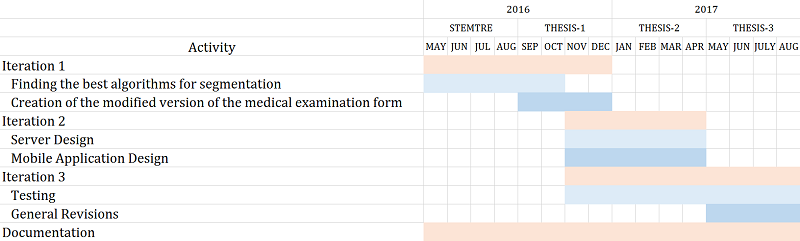
\includegraphics{gant.png}      %-- include image file named as "disneychart.png" 
	\caption{Gantt Chart of Activities}
	\label{fig:disneystock}
\end{figure}





